\documentclass[a4paper,12pt]{article}

\usepackage[utf8]{inputenc}
\usepackage[english]{babel}
\usepackage{hyperref}
\usepackage{fontenc}
\usepackage{graphicx}
\usepackage{makeidx}
\usepackage{color}
\usepackage{multirow}
\usepackage{tabularx}
\usepackage{longtable}
\usepackage{url}
\usepackage{titlesec}
\usepackage{listings}
\usepackage{xcolor}
\usepackage{colortbl}
\usepackage{geometry}

\geometry{
    a4paper,
    left=25mm,
    right=25mm,
    top=30mm,
    bottom=30mm,
 }

%%%%%%%%%%%%%%%%%%%%%%%%%%%%%
%%%%%%% CONFIGURATION %%%%%%%
%%%%%%%%%%%%%%%%%%%%%%%%%%%%%
%%%%%%%%%%%%%%%%%%%%%%%%%%%%%%%%%%%%%%
%%%%%%% SECTION CONFIGURATIONS %%%%%%%
%%%%%%%%%%%%%%%%%%%%%%%%%%%%%%%%%%%%%%
\newcommand{\sectionbreak}{\clearpage}

\setcounter{secnumdepth}{5}

\titleformat{\paragraph}
{\normalfont\normalsize\bfseries}{\theparagraph}{1em}{}
\titlespacing*{\paragraph}
{0pt}{3.25ex plus 1ex minus .2ex}{1.5ex plus .2ex}


%%%%%%%%%%%%%%%%%%%%%%%%%%%%%%%%%%%%%%
%%%%%%% LISTINGS CONFIGURATION %%%%%%%
%%%%%%%%%%%%%%%%%%%%%%%%%%%%%%%%%%%%%%
\definecolor{mybg}{rgb}{1,1,0.8}
\definecolor{mysoftblue}{rgb}{0.6,0.729,0.867}
\definecolor{mygreen}{rgb}{0,0.6,0}
\definecolor{mygray}{rgb}{0.5,0.5,0.5}
\definecolor{mymauve}{rgb}{0.58,0,0.82}

\lstset{ %
  backgroundcolor=\color{mysoftblue},    % choose the background color; you must add \usepackage{color} or \usepackage{xcolor}
  basicstyle=\ttfamily\scriptsize,        % the size of the fonts that are used for the code
  breakatwhitespace=false,         % sets if automatic breaks should only happen at whitespace
  breaklines=true,                 % sets automatic line breaking
  captionpos=b,                    % sets the caption-position to bottom
  commentstyle=\color{mygreen},    % comment style
  deletekeywords={...},            % if you want to delete keywords from the given language
  escapeinside={\%*}{*)},          % if you want to add LaTeX within your code (example: \%* int v; *) )
  extendedchars=true,              % lets you use non-ASCII characters; for 8-bits encodings only, does not work with UTF-8
  frame=single,                    % adds a frame around the code (none, single)
  keepspaces=true,                 % keeps spaces in text, useful for keeping indentation of code (possibly needs columns=flexible)
  keywordstyle=\color{blue},       % keyword style
  language=Java,                   % the language of the code
  otherkeywords={*,...},           % if you want to add more keywords to the set
  numbers=none,                    % where to put the line-numbers; possible values are (none, left, right)
  numbersep=5pt,                   % how far the line-numbers are from the code
  numberstyle=\tiny\color{mygray}, % the style that is used for the line-numbers
  rulecolor=\color{black},         % if not set, the frame-color may be changed on line-breaks within not-black text (e.g. comments (green here))
  showspaces=false,                % show spaces everywhere adding particular underscores; it overrides 'showstringspaces'
  showstringspaces=false,          % underline spaces within strings only
  showtabs=false,                  % show tabs within strings adding particular underscores
  stepnumber=2,                    % the step between two line-numbers. If it's 1, each line will be numbered
  stringstyle=\color{mymauve},     % string literal style
  tabsize=2,                       % sets default tabsize to 2 spaces
  title=\lstname,                  % show the filename of files included with \lstinputlisting; also try caption instead of title
  aboveskip=20pt,                  % space left avobe the listing
  belowskip=0pt,                   % space left below the listing
  columns=fullflexible             % to allow automatic copy from listings
}


%%%%%%%%%%%%%%%%%%%%%%%%%%%%%%%%%%%
%%%%%%% OTHER CONFIGURATION %%%%%%%
%%%%%%%%%%%%%%%%%%%%%%%%%%%%%%%%%%%

% Horizontal line
\newcommand{\HRule}{
  \rule{\linewidth}{0.5mm}
}

% Color box for comments
\newcommand{\colorComment}[1]{
\begin{table}[h]
    \centering
    \begin{tabular}{p{0.8\textwidth}}
        \cellcolor{orange}\begin{center}
	  #1 \\
        \end{center}
        \\
    \end{tabular}
\end{table}
}
\title{COMP Superscalar}
\author{MareNostrum Manual}
\date{Version 1.4}


%%%%%%%%%%%%%%%%%%%%%%%%%%%%%
%%%%%%%% DOCUMENT %%%%%%%%%%%
%%%%%%%%%%%%%%%%%%%%%%%%%%%%%
\begin{document}

  %%%%%%%%%%%% TITLE PAGE %%%%%%%%%%%%%
  \hypersetup{pageanchor=false}
  \begin{titlepage} 
    \begin{center} 
      
\includegraphics[width=0.3\textwidth]{./Figures/Logos/degradado-naranja-compss.jpg}~\\[1cm] 
      \textsc{\LARGE COMP Superscalar}\\[1.5cm] 
      
      \HRule \\[0.4cm] 
      { \huge \bfseries COMPSs at BSC \\[0.4cm] }
      { \large \bfseries MareNostrum 3 Manual \\[0.4cm] } 
      \HRule \\[1.5cm] 

      { \large \textsc{Version: 1.3 }} \\[0.3cm]
      { \large \today } 
      
      \vfill 
      % Bottom of the page
      
\includegraphics[width=0.5\textwidth]{./Figures/bsc_280.jpg}~\\[1cm]
    \end{center} 
  \end{titlepage}
  \hypersetup{pageanchor=true}
  
  %%%%%%%% REFERENCE NOTES %%%%%%%%%%
  {
    This manual only provides information about the COMPSs usage at MareNostrum. Specifically, it details the available COMPSs modules,
    how to load them and how to create and track COMPSs jobs. 
    \newline
    
    If you want to install COMPSs on your local machine please refer to the \textit{COMPSs Installation Manual} available at our
    webpage \url{http://compss.bsc.es}.
    
    For further information about the application's execution please refer to the \textit{COMPSs User Manual: Application execution
    guide} available at \url{http://compss.bsc.es} .
    
    For further information about the application's development please refer to the \textit{COMPSs User Manual: Application development
    guide} available at \url{http://compss.bsc.es/} .
    
    For full COMPSs example application (codes, execution commands, results, logs, etc.) please refer to the \textit{COMPSs Sample 
    Applications} available at \url{http://compss.bsc.es/} .
  }
  
  %%%%%%%% TABLE OF CONTENTS %%%%%%%%%%
  \pagenumbering{roman}
  \setcounter{tocdepth}{6}
  \tableofcontents
  %\listoffigures
  %\listoftables
    
  \newpage

  %%%%%%%%%%%%% CONTENTS %%%%%%%%%%%%%%
  \pagenumbering{arabic}
    
  \section{COMP Superscalar (COMPSs)}
\label{sec:Introduction}

COMP Superscalar (COMPSs) is a programming model which aims to ease the development of applications for distributed infrastructures, such as Clusters, Grids and Clouds. COMP superscalar also features a runtime system that exploits the inherent parallelism of applications at execution time.

For the sake of programming productivity, the COMPSs model has four key characteristics:

\begin{itemize}
 
 \item  {\bf Sequential programming:} COMPSs programmers do not need to deal with the typical duties of parallelization and distribution, such as thread creation and synchronization, data distribution, messaging or fault tolerance. Instead, the model is based on sequential programming, which makes it appealing to users that either lack parallel programming expertise or are looking for better programmability.
 
 \item  {\bf Infrastructure unaware:} COMPSs offers a model that abstracts the application from the underlying distributed infrastructure. Hence, COMPSs programs do not include any detail that could tie them to a particular platform, like deployment or resource management. This makes applications portable between infrastructures with diverse characteristics.
 
 \item  {\bf Standard programming languages:} COMPSs is based on the popular programming language Java, but also offers language bindings for Python and C/C++ applications. This facilitates the learning of the model, since programmers can reuse most of their previous knowledge.
 
 \item  {\bf No APIs:} In the case of COMPSs applications in Java, the model does not require to use any special API call, pragma or construct in the application; everything is pure standard Java syntax and libraries. With regard the Python and C/C++ bindings, a small set of API calls should be used on the COMPSs applications.

\end{itemize}


           
  \section{COMPSs Modules}
\label{sec:Modules}


\subsection{Available modules}
COMPSs is configured in MareNostrum (MN3) as a Linux Module. Type \textit{module available COMPSs} to list the available COMPSs modules 
through Linux Module configuration and \textit{module load $COMPSs/<version>$} to load it.
\begin{lstlisting}[language=bash]
$ module available COMPSs
---------- /apps/modules/modulefiles/tools ----------
COMPSs/0.0                          
COMPSs/0.1
COMPSs/0.2_Nested
COMPSs/1.1.2_gpfs
COMPSs/1.1.2_scratch
COMPSs/1.2 
COMPSs/1.3

COMPSs/release(default)
COMPSs/trunk


$ module load COMPSs/release
load java/1.7.0u55 (PATH, MANPATH, JAVA_HOME, JAVA_ROOT, JAVA_BINDIR, 
                    SDK_HOME, JDK_HOME, JRE_HOME)
load MKL/11.0.1 (LD_LIBRARY_PATH)
load PYTHON/2.7.3 (PATH, MANPATH, LD_LIBRARY_PATH, C_INCLUDE_PATH)
load COMPSs/release (PATH, MANPATH, IT_HOME)
\end{lstlisting}

The following command can be run to check if the correct COMPSs version has been loaded:
\begin{lstlisting}[language=bash]
$ runcompss --version
COMPSs version 1.3

\end{lstlisting}

\subsection{Configuration}
The COMPSs module contains \textbf{all} the COMPSs dependencies, including Java, Python and MKL. Modifying any of these dependencies
can cause execution failures and thus, we \textbf{do not} recomend to change them. Before running any COMPSs job please check your 
environment and, if needed, comment out any line inside the \textit{.bashrc} file loading custom COMPSs, Java, Python and/or MKL
modules.

The COMPSs module needs to be loaded in all the nodes that will run COMPSs jobs. Consequently, the \textit{module load} \textbf{must}
be included in your \textit{.bashrc} file. To do so, please run the following command with the corresponding COMPSs version:
\begin{lstlisting}[language=bash]
$ cat "module load COMPSs/release" >> ~/.bashrc
\end{lstlisting}

Log out and back in again to check that the file has been correctly edited. The next listing shows an example of the
output generated by well loaded COMPSs installation. 
\begin{lstlisting}[language=bash]
$ exit
$ ssh USER@mn1.bsc.es
load java/1.7.0u55 (PATH, MANPATH, JAVA_HOME, JAVA_ROOT, JAVA_BINDIR, 
                    SDK_HOME, JDK_HOME, JRE_HOME)
load MKL/11.0.1 (LD_LIBRARY_PATH)
load PYTHON/2.7.3 (PATH, MANPATH, LD_LIBRARY_PATH, C_INCLUDE_PATH)
load COMPSs/trunk (PATH, MANPATH, IT_HOME)

$ runcompss --version
COMPSs version 1.3
\end{lstlisting}

\colorComment{Please remember that COMPSs runs in several nodes and your current enviroment is not exported to them. Thus, all the 
needed environment variables \textbf{must} be loaded through the \textit{.bashrc} file.}


          
  \section{COMPSs Jobs}
\label{sec:Jobs}

\subsection{Submiting COMPSs jobs}
COMPSs jobs can be easily submited by running the \textbf{enqueue\_compss} command. This command allows to configure any 
\textbf{runcompss} option and some particular queue options such as the queue system, the number of nodes, the wallclock time,
the master working directory, the workers working directory and number of tasks per node.

Next, we provide detailed information about the \textit{enqueue\_compss} command:
\begin{lstlisting}[language=bash]
$ enqueue_compss --help
Usage: /apps/COMPSs/1.3/Runtime/scripts/user/enqueue_compss 
         [queue_system_options] [COMPSs_options] 
         application_name application_arguments

* Options:
  General:
    --help, -h                              Print this help message
  
  Queue system configuration:
    - -exec_time=<minutes>                  Expected execution time of 
                                            the application (in minutes)
                                            Default: 10
                                            
    - -num_nodes=<int>                      Number of nodes to use
                                            Default: 2
                                            
    - -num_switches=<int>                   Maximum number of different switches.
                                            Select 0 for no restrictions.
                                            Maximum nodes per switch: 18
                                            Only available for at least 4 nodes. 
                                            Default: 0 
                                            
    - -queue_system=<name>                  Queue system to use: lsf | pbs | slurm
                                            Default: lsf
    - -queue=<name>                         Queue name to submit the job. 
                                            Depends on the queue system.
                                            For example (MN3): bsc_cs | bsc_debug
                                                | debug | interactive
                                            Default: default
                                            
    - -job_dependency=<jobID>               Postpone job execution until the job
                                            dependency has ended.
                                            Default: None
                                            
    - -tasks_per_node=<int>                 Maximum number of simultaneous
                                            tasks running on a node
                                            Default: 16
                                            
    - -master_working_dir=<path>            Working directory of the application
                                            Default: .
                                            
    - -worker_working_dir=<name>            Worker directory. Use: scratch | gpfs
                                            Default: scratch
                                            
    - -tasks_in_master=<int>                Maximum number of tasks that the master
                                            node can run as worker. Cannot exceed 
                                            tasks_per_node.
                                            Default: 0
                                            
    - -network=<name>                       Communication network for transfers:
                                            default | ethernet | infiniband | data.
                                            Default: infiniband
          
          
  Runcompss delegated parameters:

  Tools enablers:
    - -graph=<bool>, - -graph, -g           Generation of the complete graph (true/false)
                                            When no value is provided it is set to true
                                            Default: false
                                            
    - -tracing=<bool>, - -tracing, -t       Generation of traces (true/false)
                                            When no value is provided it is set to true
                                            Default: false
                                            
    - -monitoring=<int>, - -monitoring, -m  Period between monitoring samples 
                                            (milliseconds)
                                            When no value is provided it is set to 2000
                                            Default: 0
                                            
  Runtime configuration options:
    - -project=<path>                       Path to the project XML file
                                            Default: /gpfs/apps/MN3/COMPSs/1.3/Runtime/
                                            configuration/xml/projects/project.xml
                                            
    - -resources=<path>                     Path to the resources XML file
                                            Default: /gpfs/apps/MN3/COMPSs/1.3/Runtime/
                                            configuration/xml/resources/resources.xml
                                            
    - -lang=<name>                          Language of the application (java/c/python)
                                            Default: java
                                            
    - -log_level=<level>, - -debug, -d      Set the debug level: off | info | debug
                                            Default: off
  Advanced options:
    - -comm=<path>                          Class that implements the adaptor 
                                            for communications
                                            Supported adaptors: 
                                            integratedtoolkit.nio.master.NIOAdaptor | 
                                            integratedtoolkit.gat.master.GATAdaptor
                                            Default: 
                                              integratedtoolkit.nio.master.NIOAdaptor
                                              
    - -library_path=<path>                  Non-standard directories to search 
                                            for libraries (e.g. Java JVM library, 
                                            Python library, C binding library) 
                                            Default: Working Directory
                                            
    - -classpath=<path>                     Path for the application classes / modules
                                            Default: Working Directory
                                            
    - -task_count=<int>                     Only for C/Python Bindings. Maximum number
                                            of different functions/methods, invoked
                                            from the application, that have been
                                            selected as tasks
                                            Default: 50
                                            
    - -uuid=<int>                           Preset an application UUID
                                            Default: Automatic random generation
                                            
    - -PyObject_conversion=<bool>           Only for Python Binding. Enable the object
                                            conversion to string when possible
                                            (true/false).
                                            Default: false
                                            
* Application name:
    For Java applications:   Fully qualified name of the application
    For C applications:      Path to the master binary
    For Python applications: Path to the .py file containing the main program
    
* Application arguments:
    Command line arguments to pass to the application. Can be empty. 
                                            
\end{lstlisting}

\subsection{Tracking COMPSs jobs}
When submitting a COMPSs job a temporal file will be created storing the job information. For example:
\begin{lstlisting}[language=bash]
$ enqueue_compss \
  --exec_time=15 \
  --num_nodes=3 \
  --queue_system=lsf \
  --tasks_per_node=16 \
  --master_working_dir=. \
  --worker_working_dir=gpfs \
  --lang=python \
  --log_level=debug \
  <APP> <APP_PARAMETERS>
  
Num Nodes:      3
Tasks per Node: 16
Tasks in Master:0
Master WD:      .
Worker WD:      gpfs
Exec-Time:      00:15
Network:        default
Library Path:   .
To COMPSs:      --lang=python --log_level=debug <APP> <APP_PARAMETERS>
Temp submit script is: /scratch/tmp/tmp.YPQKths559

$ cat /scratch/tmp/tmp.YPQKths559
#!/bin/bash
#
#BSUB -cwd . 
#BSUB -oo compss_3_%J.out
#BSUB -eo compss_3_%J.err
#BSUB -n 3
#BSUB -R"span[ptile=1]" 
#BSUB -J COMPSs
#BSUB -W 00:15 
...
\end{lstlisting}

In order to trac the jobs state users can run the following command:
\begin{lstlisting}[language=bash]
$ bjobs
JOBID  USER   STAT  QUEUE  FROM_HOST  EXEC_HOST  JOB_NAME  SUBMIT_TIME
XXXX   bscXX  PEND  XX     login1     XX         COMPSs    Month Day Hour
\end{lstlisting}

The specific COMPSs logs are stored under the \textit{~/.COMPSs/} folder; saved as a local \textit{runcompss} execution. For further 
details please check \textit{COMPSs User Manual: Application Execution} available at our webpage \url{http://compss.bsc.es} .

  
  \section{Enabling COMPSs Monitor}
\label{sec:Monitor}

\subsection{Configuration}

As supercomputer nodes are connection restricted, the better way to enable the \textit{COMPSs Monitor} is from the users local machine. 
To do so please install the following packages:
\begin{itemize}
 \item COMPSs Runtime
 \item COMPSs Monitor
 \item sshfs
\end{itemize}

For further details about the COMPSs packages installation and configuration please refer to the \textit{COMPSs Installation Manual} 
available at our webpage \url{http://compss.bsc.es} . If you are not willing to install COMPSs in your local machine please consider
to download our Virtual Machine available at our webpage. 
\newline

Once the packages have been installed and configured, users need to mount the sshfs directory as follows. The \verb|SC_USER| stands for 
your supercomputer's user, the \verb|SC_ENDPOINT| to the supercomputer's public endpoint and the \verb|TARGET_LOCAL_FOLDER| to 
the local folder where you wish to deploy the supercomputer files):

\begin{lstlisting}[language=bash]
compss@bsc:~$ scp $HOME/.ssh/id_dsa.pub ${SC_USER}@mn1.bsc.es:~/id_dsa_local.pub
compss@bsc:~$ ssh SC_USER@SC_ENDPOINT 
                  "cat ~/id_dsa_local.pub >> ~/.ssh/authorized_keys; 
                  rm ~/id_dsa_local.pub"
compss@bsc:~$ mkdir -p TARGET_LOCAL_FOLDER/.COMPSs
compss@bsc:~$ sshfs -o IdentityFile=$HOME/.ssh/id_dsa -o allow_other 
                   SC_USER@SC_ENDPOINT:~/.COMPSs 
                   TARGET_LOCAL_FOLDER/.COMPSs
\end{lstlisting}

Whenever you wish to unmount the sshfs directory please run:

\begin{lstlisting}[language=bash]
compss@bsc:~$ sudo umount TARGET_LOCAL_FOLDER/.COMPSs
\end{lstlisting}


\subsection{Execution}
Access the COMPSs Monitor through its webpage (\url{http://localhost:8080/compss-monitor} by default) and log in with the 
\verb|TARGET_LOCAL_FOLDER| to enable the COMPSs Monitor for MareNostrum. 

\colorComment{Please remember that to enable \textbf{all} the COMPSs Monitor features applications must be ran with the \textit{-m}
flag. For further information please check the \textit{COMPSs User Manual: Application Execution} available at our webpage
\url{http://compss.bsc.es} .}

\newpage

~ \newline

Figure \ref{fig:mn_monitor1} illustrates how to login and Figure \ref{fig:mn_monitor2} shows the COMPSs Monitor
main page for an application run inside a Supercomputer. 

~ \newline

\begin{figure}[!htb]
  \centering
    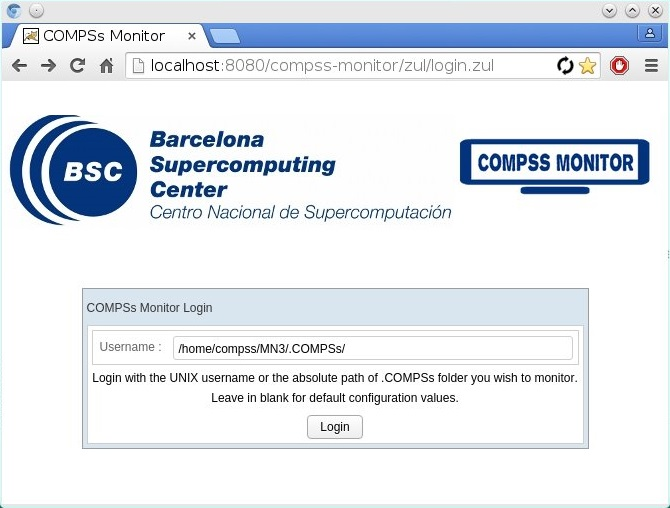
\includegraphics[width=0.75\textwidth]{./Sections/6_Monitor/Figures/mn_monitor1.jpeg}
    \caption{COMPSs Monitor login for Supercomputers}
    \label{fig:mn_monitor1}
\end{figure}

\newpage

\begin{figure}[!htb]
  \centering
    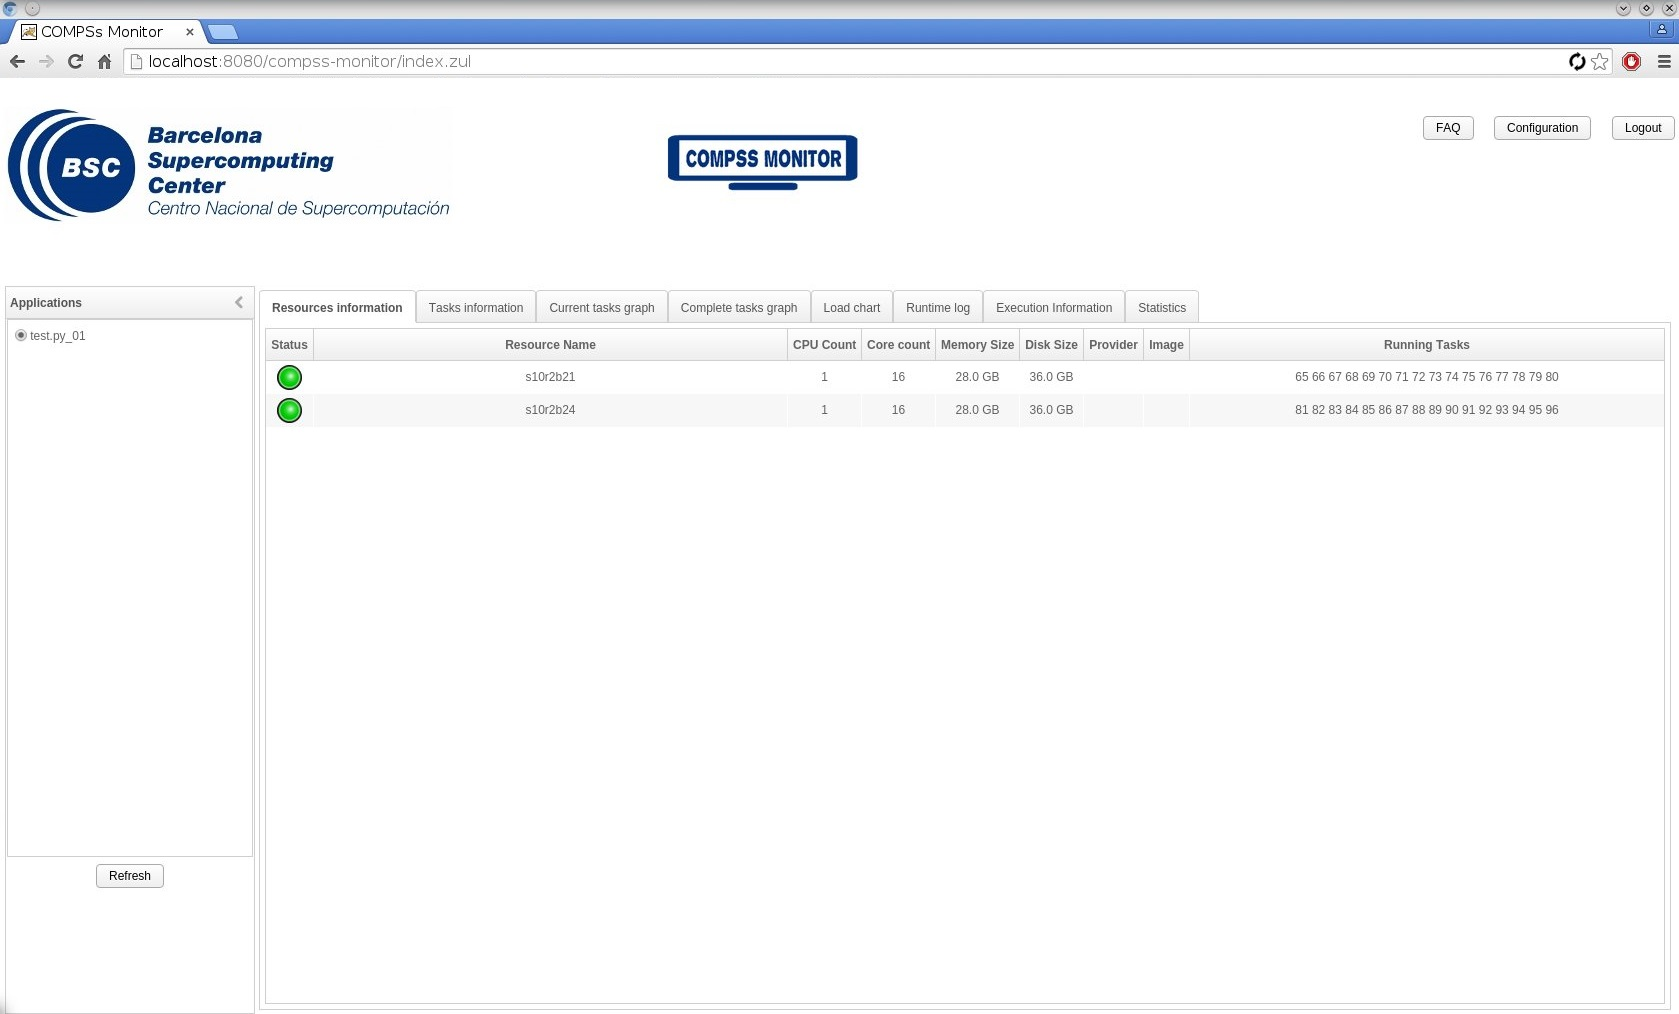
\includegraphics[width=\textwidth]{./Sections/6_Monitor/Figures/mn_monitor2.jpeg}
    \caption{COMPSs Monitor main page for a test application at Supercomputers}
    \label{fig:mn_monitor2}
\end{figure}

  
  %%%%%%%%%%%%% END PAGE %%%%%%%%%%%%%%
  \newpage

  \vspace*{\fill} 
  \begin{center}
    \large { Please find more details on the COMPSs framework at }
    \huge{\url{http://compss.bsc.es}}
  \end{center}    
  \vspace*{\fill} 
           
\end{document}
